\chapter[RicoSLAM: Framework for Localization and Mapping in Dynamic
Environments]{RicoSLAM: Framework for Localization and Mapping in
Dynamic Environments}\label{appx:ricoslam}
\begin{description}[leftmargin=1cm,style=nextline,font=\normalfont]
\item[\cite{sousa:ral:2026}] \fullcite{sousa:ral:2026}.
\end{description}

\noindent
The manuscript reproduced below is complete and awaiting the final feedback of
the co-authors before submission. Relative to \chapref{chap:slam}, it narrows
the scope to the online \gls{slam} operation and to the dynamics removal
mechanisms, leaving out the \gls{gba} formulations of \secref{sec:slam:gba},
and extends the experimental evaluation with the
Cartographer~\cite{hess:icra:2016} baseline and with the total execution time
of every framework processing the same sequences on the same hardware.

\cleardoublepage

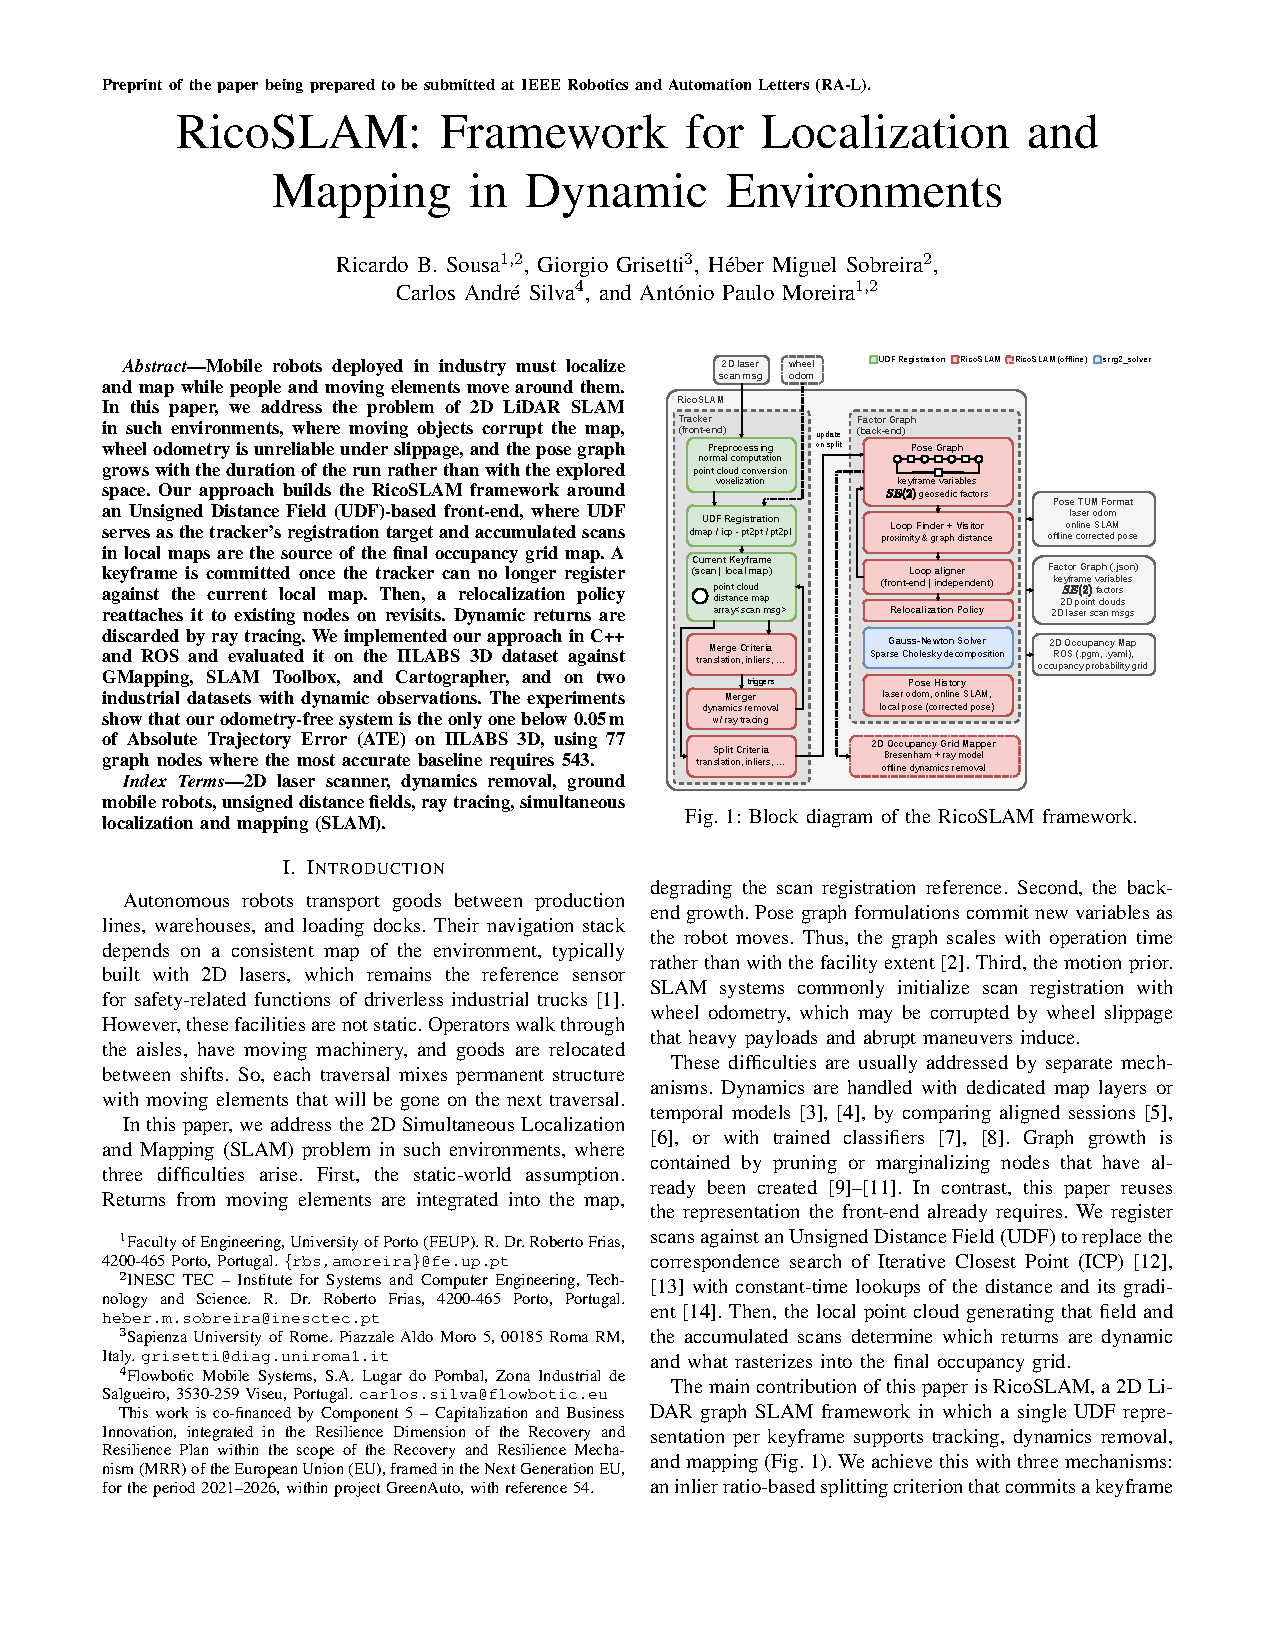
\includepdf[pages={-}]{appendices/files/ricoslam.pdf}
